\section{Implementierung und Deployment}
\subsection{Auswahl der Technologien}
Die Auswahl der geeigneten Technologien für die Entwicklung des innovativen 
Studiengangsfinders wurde so gewählt, um eine effiziente und interaktive Lösung
zu gewährleisten. Besonders wichtig ist die Nutzbarkeit auf
Smartphones und Desktop-Geräten, wodurch sich außerdem neue Herausforderungen
hinsichtlich der Bedienung ergeben. Im Folgenden werden die Hauptkomponenten des
Technologiestacks und ihre jeweiligen Funktionen erläutert.

\subsubsection{Pixi.js - Interaktive Grafik}
Für die Darstellung der interaktiven Grafik wurde Pixi.js gewählt. Pixi.js ist
ein leistungsstarkes WebGL-Rendering-Framework, das eine schnelle und
reibungslose Darstellung von Grafiken ermöglicht. \parencite{pixijs_pixijs_2023} Die
Entscheidung für Pixi.js basiert auf seiner Effizienz bei der Verarbeitung
komplexer 2D-Grafiken und seiner Fähigkeit, eine ansprechende Benutzererfahrung
zu bieten.

Neben Pixi.js wurden verschiedene weitere Bibliotheken betrachtet:
\begin{itemize}
    \item three.js: WebGL 3D-Framework
    \item D3.js: 2D-Datenvisualisierungsbibliothek
    \item Chart.js: HTML5-Bibliothek für Diagramme
    \item Paper.js: HTML5-Bibliothek für Animationen und interaktive Grafiken
    \item Fabric.js: 2D-Canvas Bibliothek
\end{itemize}

% TODO: Quellen für die "Forenthreads" gegen die Frameworks etc verlinken

Der Studiengangsfinder erfordert eine 2D-Grafikdarstellung, weshalb
\textit{three.js}, das auf 3D-Visualisierungen spezialisiert ist, nicht als
geeignete Grundlage gewählt wurde. \parencite{threejs_threejs_2023}

Die Entscheidung gegen die Verwendung von \textit{D3.js} wurde aufgrund
von Bedenken bezüglich der Dokumentation und der Wahrnehmung in der 
Entwicklergemeinschaft getroffen. Die unvollständige Dokumentation und
bestehende Forenthreads, die die Relevanz von D3.js in Frage stellen, könnten zu
potenziellen Schwierigkeiten bei der Entwicklung und zukünftigen Wartungen
führen. \parencite{bostock_d3js_2023}

% d3js-trend, d3js-trend-2

Aufgrund der festgestellten Einschränkungen in der Flexibilität von
\textit{Chart.js} wurde gegen die Verwendung der Bibliothek entschieden. Obwohl
Chart.js die Erstellung einer Vielzahl von Diagrammen ermöglicht, hat sich
gezeigt, dass die Anpassbarkeit eingeschränkt ist. \parencite{etimberg_chartjs_2023}

Basierend auf der wahrgenommenen Inaktivität des Projekts und den festgestellten 
Einschränkungen in Bezug auf Event-Handler wurde entschieden, \textit{Paper.js}
nicht zu verwenden. \parencite{lehni_paperjs_2023} Die begrenzten Event-Handler schränken
die Interaktionsmöglichkeiten ein, was im Kontext des Studiengangsfinders, der
eine umfassende Benutzerinteraktion für Smartphone und Desktop-Gerät erfordert,
als unzureichend erachtet wurde. \parencite{etimberg_paperjs_2023}

Obwohl \textit{Fabric.js} als vielversprechende Alternative erschien, wurde
Pixi.js aufgrund mehrerer Faktoren bevorzugt \parencite{zaytsev_fabricjs_2023}. Der
professionellere Website-Auftritt von Pixi.js trug dazu bei, das Vertrauen in
die Zuverlässigkeit und Wartbarkeit des Frameworks zu stärken. Ein weiterer
bedeutender Punkt ist die Anzahl der GitHub-Sterne in Relation zu der Anzahl an
\textit{offenen Issues}, die Pixi.js aufweist. Eine höhere Anzahl an
GitHub-Sternen mit gleichzeitig weniger offenen Issues, deutet oft auf eine
größere und aktivere Entwicklergemeinschaft hin, was wiederum auf
kontinuierliche Weiterentwicklung und Wartung schließen lässt.
\parencite{batista_github_2023}

\subsubsection{Python - Berechnung der Positionen}
Die Berechnung der Positionen für die Studiengänge basiert, wie im Abschnitt
\ref{sec:MDS} erläutert, auf dem Multidimensionalen Skalierungsalgorithmus
(MDS), der in Python implementiert ist. Der Algorithmus verarbeitet eine
strukturierte CSV-Datei, die alle relevanten Informationen zu den Studiengängen,
Feldern und Meta-Informationen (wie z.B. Fakultätszugehörigkeit) enthält. Dieser
Datensatz bildet die Grundlage für die Positionsbestimmung im zweidimensionalen
Raum.

Hierzu wird ein Python-Skript entwickelt, welches die CSV-Datei einliest und
schließlich den MDS-Algorithmus auf den Daten anwendet. Im Verlauf der
Arbeit wurde eine anfängliche Eigenimplementierung des MDS-Algorithmus in
Betracht gezogen. Folgender Ausschnitt eines Quellcodes beinhaltet die für diese
Arbeit entwickelte Eigenimplementierung, basierend auf dem im Abschnitt
\ref{sec:MDS} genau erläuterten Ablauf:

\begin{lstlisting}[style=Python]
    import numpy as np

    def calculate_distance_matrix(X):
        ...

    def read_data_from_csv():
        ...

    def mds(self):
        # Reads data from CSV file and transforms it to number rows
        X = self.read_data_from_csv()

        # Calculates distance matrix
        M = self.calculate_distance_matrix(X)

        # Double centered matrix
        n = 11 # Number of subjects
        I = np.identity(n) # Identity matrix
        Jn = np.ones((n, n)) # Matrix Jn of all ones
        C = I - (1/n) * Jn # Calculate centering matrix C
        B = -0.5 * np.dot(np.dot(C, np.array(M)), C) # Calculate the double centered matrix B

        # Eigenvalues, Eigenvectors
        m = 2  # number of dimensions (2D)
        eigenvalues, eigenvectors = np.linalg.eig(B) # Perform eigenvalue decomposition

        # Sort eigenvalues and corresponding eigenvectors in descending order
        sorted_indices = np.argsort(eigenvalues)[::-1]
        eigenvalues = eigenvalues[sorted_indices]
        eigenvectors = eigenvectors[:, sorted_indices]

        # Select the top m eigenvalues and corresponding eigenvectors
        top_m_eigenvalues = eigenvalues[:m]
        top_m_eigenvectors = eigenvectors[:, :m]

        # Calculate the square root of the diagonal matrix
        sqrt_Lambda_m = np.sqrt(np.diag(top_m_eigenvalues))

        # Compute the matrix X using the formula
        X_transformed = np.dot(top_m_eigenvectors, sqrt_Lambda_m)

        return X_transformed
\end{lstlisting}

Die Methode \code{calculate\_distance\_matrix} berechnet die Distanzmatrix,
welche für den Ablauf des Programms essenziell ist. Der Code dazu wird an
dieser Stelle ausgespart, da er bereits in Abschnitt \ref{sec:distanzmatrix}
vollständig spezifiziert wurde. Außerdem ausgespart ist die Methode
\code{read\_data\_from\_csv()}, welche die Eingabedatei einliest, analysiert und
schließlich die zur Berechnung benötigten Zahlen-Arrays zurückgibt. Wie in Zeile
1 des Quellcodes ersichtlich, wird zur Berechnung der mathematischen Gleichungen
die Programmbibliothek NumPy verwendet. \parencite{team_numpy_2023}

Die Entwicklung und Umsetzung dieser eigenen Lösung erwies
sich jedoch als äußerst anspruchsvoll, da sie zahlreiche subtile mathematische
Nuancen berücksichtigen müsste. Angesichts dieser Komplexität wurde die
Entscheidung getroffen, auf die bewährte und leistungsstarke
SciKit-Learn-Bibliothek zurückzugreifen. Die Verwendung dieser etablierten
Implementierung ermöglicht eine präzise und effiziente Lösung, wobei der Fokus
auf den zentralen Fragestellungen der Masterarbeit liegt. Außerdem gewährleistet
die Einbindung von SciKit-Learn neben der Robustheit der MDS-Umsetzung, auch die
Reduktion der Entwicklungskomplexität im Hinblick auf die
Algorithmusimplementierung. \parencite{developers_scikit}

Das Ergebnis des Skripts sind Koordinaten für jeden Studiengang im
zweidimensionalen Raum. Diese Koordinaten werden anschließend zusammen mit den
vorher eingelesenen Meta-Daten zu den Studiengängen in JSON-Dateien gespeichert,
die schließlich vom Backend über eine Webschnittstelle bereitgestellt werden.

Der Vorteil bei der Speicherung der berechneten Positionen in Form von
JSON-Dateien liegt darin, dass die Daten wesentlich seltener geändert werden,
als die Website aufgerufen wird. Somit wird effektiv Rechenleistung und Strom
gespart. Gleichzeitig erhöht
dieses Vorgehen die Performance der Website. Zur Festigung dieser These werden
die Google Suchtrends von 2021 zum Suchbegriff \glqq OTH Regensburg
Studiengänge\grqq{} herangezogen (siehe Anhang
\ref{appendix:google-search-trends}). Die Trends zeigen eine Jahressumme von
1194 Suchanfragen. Die Anzahl an Suchanfragen lassen sich nicht 1:1 in
Seitenaufrufe projizieren, verdeutlichen aber dennoch einen ungefähren
Richtwert. Die Datengenerierung hingegen wird nach mündlicher Zusage von
Frau Rösel (Vizepräsidentin der OTH-Regensburg) nur bei größeren Änderungen an den
Inhalten von Studiengängen, oder beim Hinzufügen bzw. Entfernen eines 
Studiengangs ausgelöst. Dies wiederum passiere meist insgesamt nur einmal pro
Jahr.

\subsubsection{Node.js - REST-API}
Wie im vorherigen Abschnitt erläutert, ist neben dem Python-Programm auch eine Webschnittstelle erforderlich. In diesem Fall wird hierfür Node.js in Kombination mit der Bibliothek Express verwendet. Node.js ist eine JavaScript-Runtime-Umgebung, die auf der V8 JavaScript Engine von Google basiert und eine serverseitige Ausführung von JavaScript ermöglicht. \parencite{foundation_nodejs_2023} Express wiederum ist ein quelloffenes Webanwendungs-Framework für Node.js. Es erleichtert die Erstellung von Webanwendungen und APIs, indem es eine Reihe von Funktionen und Tools für den Aufbau von Webanwendungen bereitstellt.
\parencite{foundation_express_2023}

Der daraus entstehende Webservice ermöglicht den Zugriff, auf die vom Python-Skript generierten Dateien, über standardisierte REST-Endpunkte.

Eine REST-API (Representational State Transfer Application Programming Interface) ist eine zustandslose Schnittstelle, die es ermöglicht, über HTTP-Methoden, wie GET, POST oder PATCH, auf Ressourcen des Systems zuzugreifen und mit ihnen zu interagieren.

\noindent
In der folgenden \autoref{table:rest-api} werden die REST-Endpunkte von StudyMap vorgestellt:
\begin{table}[!ht]
    \centering
    \begin{tabular}{|l|l|l|l|}
    \hline
    \textbf{Methode} & \textbf{Pfad}             & \textbf{Rückgabewert} \\ \hline
    \textbf{GET}     & /data/history             & application/json      \\ \hline
    \textbf{PATCH}   & /data/history/restore/:id & application/json      \\ \hline
    \textbf{GET}     & /data/generate?mode=:mode & application/json      \\ \hline
    \textbf{GET}     & /data/download/:version   & application/zip       \\ \hline
    \textbf{POST}    & /data/upload              & application/json      \\ \hline
    \end{tabular}

    \caption{StudyMap-API: REST-Endpunkte}
    \label{table:rest-api}
\end{table}

\noindent
Beschreibung der in \autoref{table:rest-api} aufgezählten Endpunkte:

\paragraph*{/data/history}
\vspace{-1.0em}
Gibt alle existierenden Datensicherungen in einem Array aus IDs aus.

\paragraph*{/data/history/restore/:id}
\vspace{-1.0em}
Stellt Datensicherung mit der ID :id wieder in die Staging-Umgebung her. :id ist ein Pfadparameter.

\paragraph*{/data/generate?mode=:mode}
\vspace{-1.0em}
Erstellt anhand der bereits hochgeladenen Dateien eine neue Version und erzeugt im Falle einer Produktivversion eine Datensicherung. :mode ist dabei ein Queryparameter mit :mode $\in$ {'staging', 'production'}.

\paragraph*{/data/download/:version}
\vspace{-1.0em}
Erstellt aus der Version :version eine .zip-Datei und erstellt daraus einen Download-Stream. Für den Pfadparameter :version gilt :version $\in$ {'staging', 'production', 'template'}.

\paragraph*{/data/upload}
\vspace{-1.0em}
Nimmt mehrere Dateien entgegen und speichert diese im Input des StudyMap-Algorithmus. Die zu hochladenden Dateien müssen im Body der HTTP-Anfrage enthalten sein. Dabei gibt es die Regeln: dataset (1 Datei), faculties (1 Datei) und details (maximal 50 Dateien). Die hochgeladenen Dateien können anschließend per Aufruf von /data/generate verarbeitet werden.

Durch die in diesem Unterkapitel beschriebene Web-Schnittstelle kann das Pixi.js-Frontend in Echtzeit die benötigten Informationen abrufen, um die interaktive Grafik der Studiengänge zu erstellen. Die klare Trennung von Backend und Frontend gewährleistet eine effiziente Datenübertragung und ermöglicht eine dynamische Aktualisierung der Grafik bei Änderungen im Datensatz.

\subsubsection{Angular - Administrationsoberfläche}
Um den im Kapitel Konzept aufgeführten Anforderungen wie Datensicherung und Trennung von Staging- und Produktivumgebung gerecht zu werden, ist die Implementierung einer Verwaltungssoftware notwendig. Um die Entwicklung möglichst zukunftssicher, d.h. leicht erweiterbar zu gestalten, wird ein sogenanntes Webframework eingesetzt.

Ein Webframework ist eine Sammlung von Bibliotheken, Tools und Technologien und bietet Programmierern ein Grundgerüst für eine dynamische Webanwendung. Neben der Zeitersparnis durch die bereits vorhandenen Bausteine hat die Verwendung eines Webframeworks den Vorteil, dass es in der Regel eine standardisierte Struktur vorgibt, die es späteren Entwicklern erleichtert, an dem Projekt weiterzuarbeiten. Generell arbeiten die meisten Frameworks nach dem DRY-Prinzip (Don't repeat yourself), was den Code schlanker und damit weniger fehleranfällig macht.
\parencite{domainfactory_beliebtesten_2023}

Für die Entwicklung der Administrationsoberfläche wurde Angular als Webframework gewählt. Der Grund für die Wahl des Frameworks liegt in seiner Verbreitung, da Angular neben dem React-Framework und Vue.js eines der meistgenutzten Frontend-Frameworks ist. \parencite{greif_state_2022}

Angular ist ein komponentenbasiertes Framework zur Erstellung von skalierbaren Webanwendungen auf Basis der Programmiersprache TypeScript. Es enthält unter anderem Bibliotheken für das Routing zwischen Seiten, dynamische Formulare, Client-Server-Kommunikation und mehr \parencite{google_inc_angular_2023}. Zusätzlich zum Angular-Framework wird ein CSS-Framework benötigt, um vordefinierte Styles und wiederverwendbare Komponenten wie z.B. Dialoge zu erhalten.

HTML steht für HyperText Markup Language und ist die Sprache des Internets. HTML ist eine Dokumentenbeschreibungssprache, mit der die Struktur von Webseiten definiert wird. Mithilfe von CSS wird dann das Layout und Aussehen der in HTML definierten Elemente (z.B. Schaltflächen) festgelegt. \parencite{mozilla_corporation_html_2023}

CSS wiederum steht für Cascading Style Sheets und definiert Darstellungsregeln für HTML-Elemente. CSS-Regeln enthalten Definitionen zu Größe, Form, Farbe, Animation und Layout der einzelnen HTML-Elemente einer Website. \parencite{mozilla_corporation_what_2024}

Im Fall von StudyMap wird Angular Material UI verwendet. Angular Material UI ist ein von Google entwickeltes CSS-Framework. Die Entscheidung für dieses Framework beruht darauf, dass es ebenso wie das Angular Framework von Google LLC entwickelt wurde und daher sehr gut parallel kombiniert werden kann. \parencite{google_llc_angular_2024}
\subsection{Architektur}
Das Gesamtbild StudyMap setzt sich aus den vorher genauer erläuterten Komponenten REST-API, Pixi.js, Python-Backend und Node.js als Webserver für alle Dienste zusammen. Dieses Kapitel beschäftigt sich mit der Architektur und der Kommunikation der einzelnen Komponenten untereinander.

Obwohl die Softwarearchitektur erst in den letzten 30 Jahren an Bedeutung gewonnen hat, ist sie ein fester Bestandteil der Softwareentwicklung und definiert wesentliche tragende Säulen des Produkts. Dabei geht die Softwarearchitektur nicht auf die internen Details einer bestimmten Komponente ein. \parencite{vogel_einleitung_2009} Sie soll komplexe Zusammenhänge übersichtlich darstellen und Fragen wie folgende beantworten:
\begin{itemize}
    \item Wie hängen die Systembausteine miteinander zusammen?
    \item Welche Schnittstellen haben die Komponenten?
    \item Worauf sind Strukturierungen und Entscheidungen zurückzuführen?
\end{itemize}

Für StudyMap ist eine Darstellung der Softwarearchitektur aus mehreren Gründen essentiell.

\paragraph*{Grund 1: Komplexität}
Die Komplexität der Software wird übersichtlicher dargestellt. Da bei der Verwendung mehrerer Programmiersprachen wie JavaScript, TypeScript und Python schnell die Übersicht über die einzelnen Komponenten verloren gehen kann, besteht die Gefahr, ineffizienten oder im schlimmsten Fall fehlerhaften Code zu produzieren. Ein weiterer Grund ist die Einarbeitung zukünftiger Entwickler.

\paragraph*{Grund 2: Einarbeitung}
Da StudyMap im Rahmen dieser Masterarbeit entsteht, ist es abzusehen, dass es immer wieder wechselnde Stakeholder und Weiterentwickler für das Projekt geben wird. Diese müssen zwangsläufig eingearbeitet werden und das Gesamtprojekt verstehen. Ein Entwickler, dem der gesamte Workspace ohne Strukturgrafik mit vier miteinander kommunizierenden Projekten präsentiert wird, könnte überfordert sein. Deshalb dient die Softwarearchitektur der effizienten Einarbeitung.

\paragraph*{Grund 3: Sicherheit}
Schließlich ist die Strukturgrafik für die Sicherheit der Hochschule von Bedeutung. StudyMap enthält einen geschützten Administrationsbereich. Es sollte im Vorfeld genau festgelegt werden, dass z.B. der Administrationsbereich nur über das VPN der Hochschule erreichbar ist, um die Wahrscheinlichkeit eines Hackerangriffs zu reduzieren. Solche Beziehungen lassen sich mithilfe der Definition einer Softwarearchitektur präzise festlegen. Außerdem benötigt man diese Darstellung explizit an der OTH-Regensburg, um einen Server vom Rechenzentrum für das Hosting von StudyMap zu erhalten. Weitere Informationen dazu finden Sie im \autoref{sec:deployment}.

\begin{figure}[H]
    \centering
    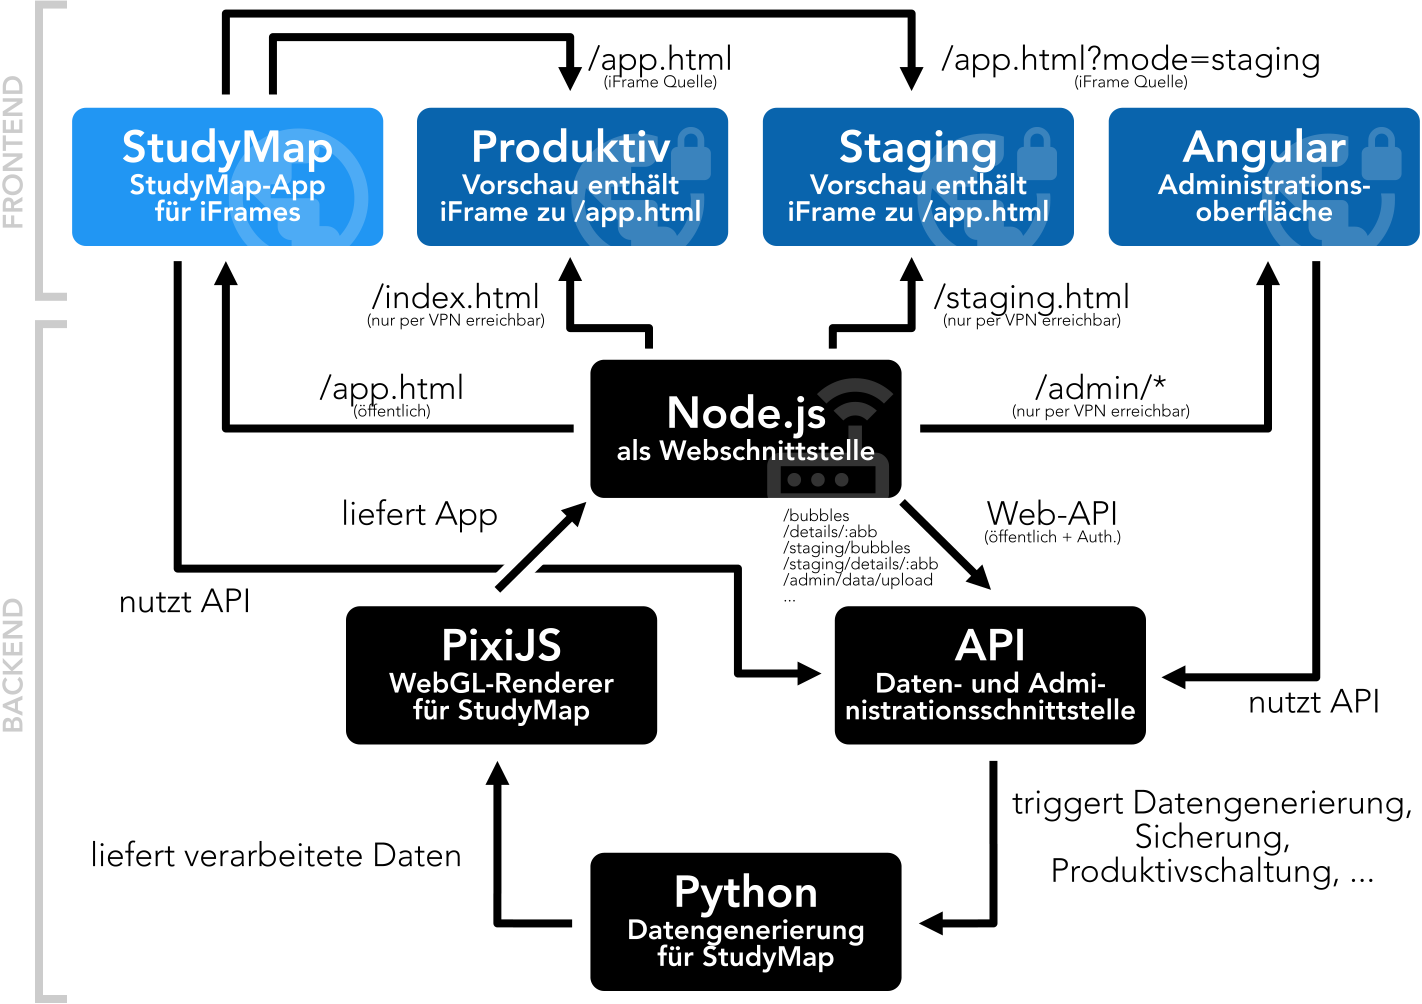
\includegraphics[width=\textwidth]{architecture}
    \caption{Softwarearchitektur von StudyMap}
    \bildquelle{Eigene Darstellung}
    \label{fig:studymap-architecture}
\end{figure}

% TODO: Describe Architektur

\subsection{Deployment}\label{sec:deployment}